\documentclass[assignment4.tex]{subfiles}
\begin{document}

\section*{2η Άσκηση}
Το πολυώνυμο παρεμβολής \textlatin{Newton} μπορεί να βρεθεί με χρήση του αλγορίθμου διηρημένων διαφορών. Συγκεκριμένα το πολυώνυμο που προκύπτει είναι της μορφής (\ref{eq:newton_poly}), όπου οι συντελεστές $a_i$ δίνονται από τις διηρημένες διαφορές (\ref{eq:divided_diff}) και $x_i,i=0,1,\dots n$ τα σημεία παρεμβολής. 

\begin{equation}
P_n(x) = a_0 + a_1(x-x_0) + \dots + a_n(x-x_0)(x-x_1)\cdots (x-x_n)
\label{eq:newton_poly}
\end{equation}

\begin{equation}
a_i = f[x_0, x_1, \dots, x_i]
\label{eq:divided_diff}
\end{equation}
Το αποτέλεσμα της παρεμβολής δίνεται στο Σχήμα \ref{fig:ex2}.
\begin{figure}[hp]
	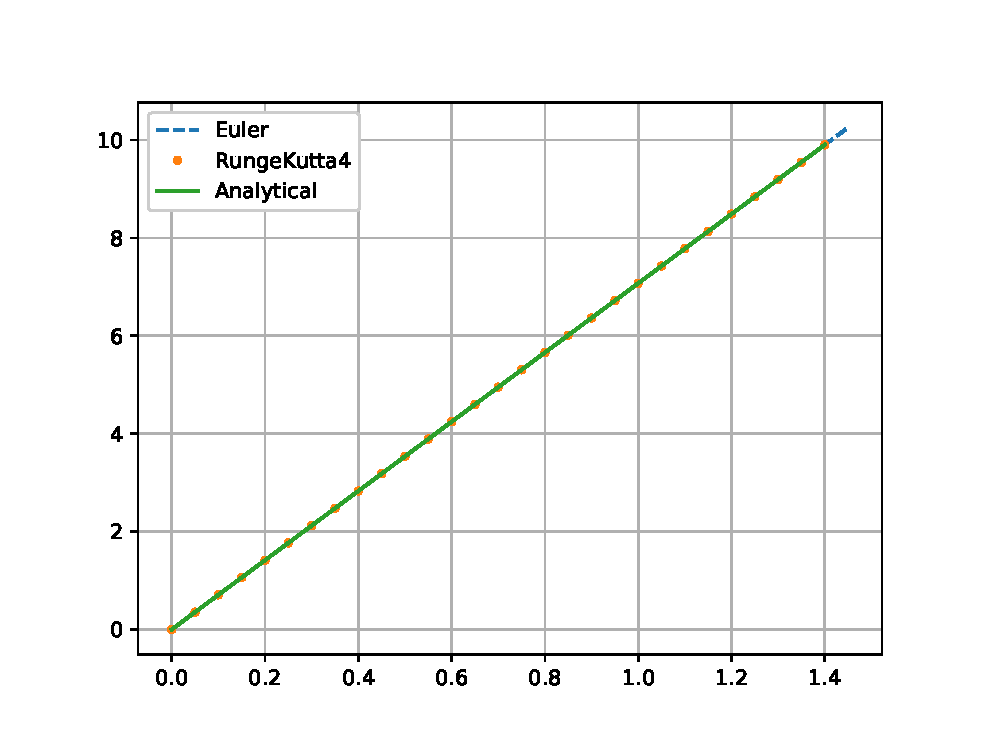
\includegraphics[width=0.9\textwidth]{ex2a.eps}
	\centering
	\caption{Παρεμβολή με πολυώνυμο \textlatin{Newton}}
	\label{fig:ex2}
\end{figure}
Σχετικά με το σφάλμα προσέγγισης $f(x)-P(x)$ στο $x\in[0,\dfrac{\pi}{2}]$, αποδεικνύεται ότι δίνεται από την εξίσωση (\ref{eq:error_interpolation}), με $\xi\in (a, b)$, όπου $a=\min[x_0, \dots x_n]$ και $b=\max[x_0, \dots x_n]$.
\begin{equation}
f(x)-p_n(x)=\frac{(x-x_0)\cdots(x-x_n)}{(n+1)!}f^{(n+1)}(\xi)
\label{eq:error_interpolation}
\end{equation}
Λαμβάνοντας την απόλυτη τιμή της (\ref*{eq:error_interpolation}) και για την δοσμένη $f(x)$ προκύπτει η (\ref{eq:actual_error}). Στο Σχήμα \ref{fig:ex2_error}, δίνεται η γραφική παράσταση του σφάλματος στο υπό εξέταση διάστημα.

\begin{equation}
\begin{split}
|f(x)-p_n(x)|&=\left|\frac{x(x-\dfrac{1}{2})(x-1)}{4!}\sin\xi\right| \rightarrow \\
&\leq \frac{|x||x-\dfrac{1}{2}||x-1|}{4!}\rightarrow \\
& \leq \frac{\dfrac{\pi}{2} (\dfrac{\pi}{2}-\dfrac{1}{2})(\dfrac{\pi}{2}-1)}{4!} \rightarrow \\
&=\frac{\pi^3-3\pi^2+2\pi}{192} \approx 0.04
\end{split}
\label{eq:actual_error}
\end{equation}

\begin{figure}[hp]
	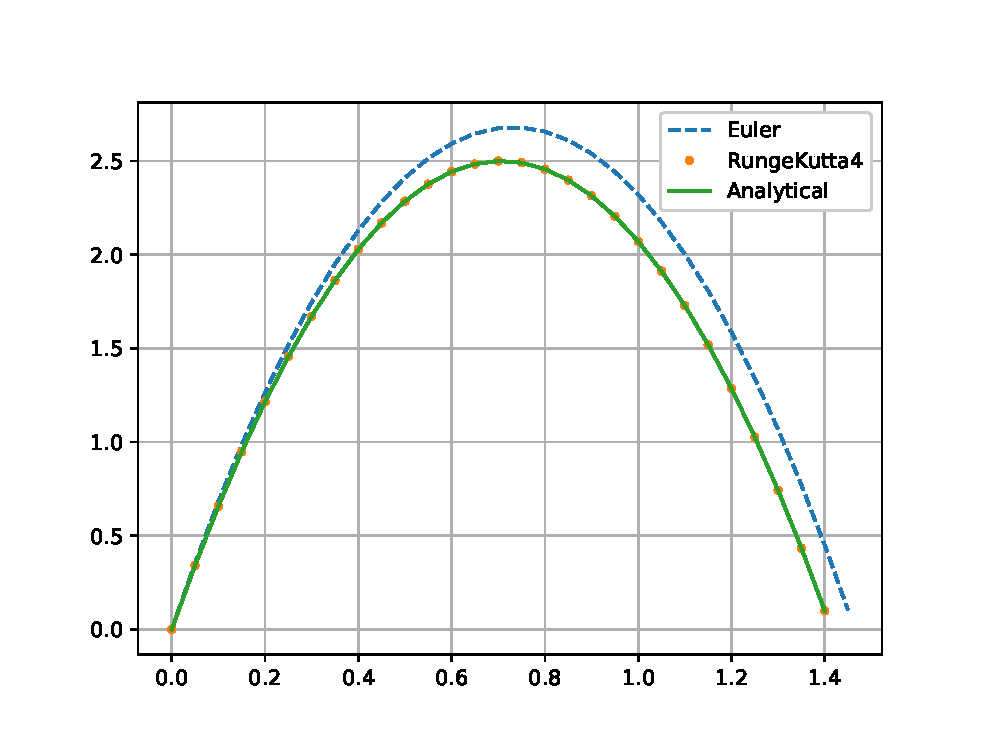
\includegraphics[width=0.7\textwidth]{ex2b.eps}
	\centering
	\caption{Παρεμβολή με πολυώνυμο \textlatin{Lagrange}}
	\label{fig:ex2_error}
\end{figure}

Παρακάτω ακολουθεί ο κώδικας που γράφτηκε σε \textlatin{Python} και έγινε χρήση της βιβλιοθήκης \textlatin{Numpy}. Ο αλγόριθμος διηρημένων διαφορών και φωλιασμένου υπολογισμού της τιμής του πολυωνύμου δίνεται στο Παράρτημα.
\selectlanguage{english}
\lstinputlisting[style=python, firstline=8]{ex2.py}
\end{document}